\documentclass{article}
\usepackage[utf8]{inputenc}


\begin{document}

\begin{center}
\caption\textbf{HERRAMIENTAS DE BUSINESS ANALITYCS}
\end{center}
\\
\begin{itemize}
\item Las 5 fuerzas de Porter:
\\Esta herramienta de análisis estratégico, ideada por el ingeniero y profesor Michael Porter en 1979, todavía sigue vigente. El modelo delimita un marco que nos permite analizar el nivel de competencia dentro de un sector para poder idear, así, una estrategia de negocio que haga rentable nuestra empresa. En este sentido, es ideal para elaborar un plan de negocio, dado que es fundamental analizar la competencia antes de crear una empresa, por lo que este modelo es especialmente interesante para emprendedores. Las cinco fuerzas de Porter son las siguientes:

- Poder de negociación de los compradores o clientes
- Poder de negociación de los proveedores o vendedores
- Amenaza de nuevos competidores
- Amenaza de productos sustitutos
- Rivalidad entre los competidores
		\begin{center}
		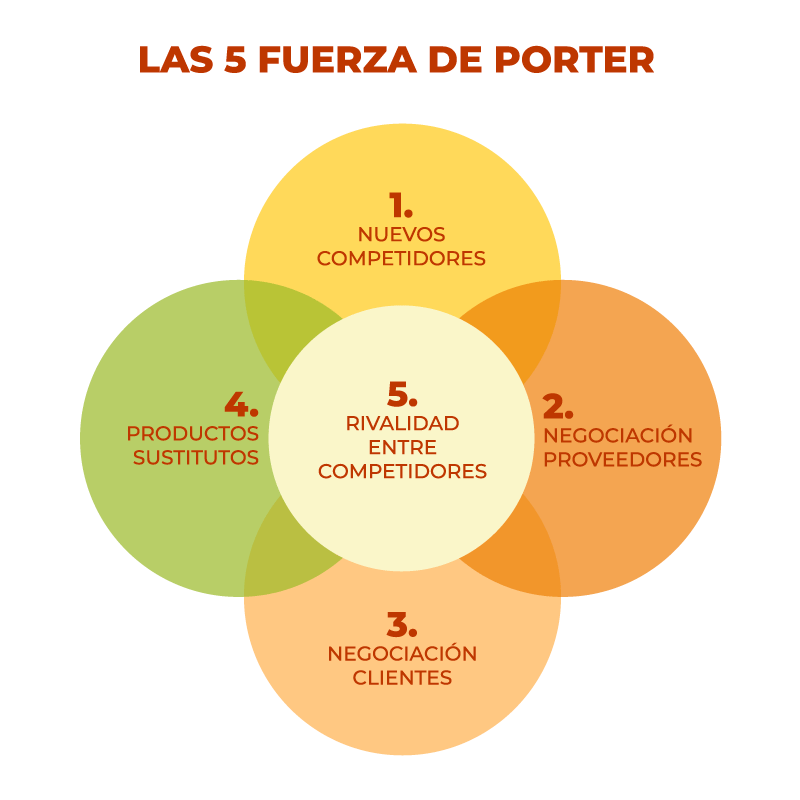
\includegraphics[width=15cm]{./Imagenes/Imagen5}
		\end{center}

	\end{itemize} 
	
	\begin{itemize}
\item Estrategia del océano azul:
\\Esta herramienta, más que para elaborar nuestro plan de negocio, es ideal para hacernos pensar y ver cómo queremos enfocar nuestra empresa. Una estrategia de océano azul es lo que puede llevar nuestra empresa al éxito. Por eso todo emprendedor debería conocer esta herramienta y, antes de montar su empresa soñada, dedicar un tiempo a pensar cuál puede ser su estrategia del océano azul.
		\begin{center}
		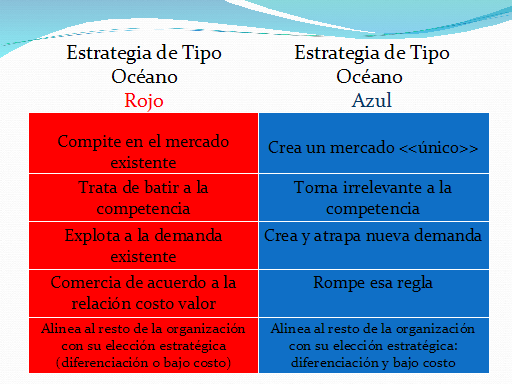
\includegraphics[width=15cm]{./Imagenes/Imagen6}
		\end{center}
	\end{itemize} 

\end{document}
